%%% LaTeX Template: Article/Thesis/etc. with colored headings and special fonts
%%%
%%% Source: http://www.howtotex.com/
%%% Feel free to distribute this template, but please keep to referal to http://www.howtotex.com/ here.
%%% February 2011
%%%
%%% Last updated September 2018 by CDM

%%%  Preamble
\documentclass[11pt,letterpaper]{article}
\usepackage[margin=1.0in]{geometry}
\usepackage[T1]{fontenc}
\usepackage[bitstream-charter]{mathdesign}
\usepackage[latin1]{inputenc}					
\usepackage{amsmath}						
\usepackage{xcolor}
\usepackage{cite}
\usepackage{hyphenat}
\usepackage{graphicx}
\usepackage{float}
\usepackage{subfigure}
\usepackage{sectsty}
\usepackage[compact]{titlesec} 
\usepackage[tablegrid]{vhistory}
\allsectionsfont{\color{accentcolor}\scshape\selectfont}

%%% Definitions
%%%%%%%%%%%%%%%%%%%%%%%%%%%%%%%%%%%%%%%%%%%%%%%%%%
% Change me to fit your team/semester information
\definecolor{accentcolor}{rgb}{0.0,0.0,0.5} 
\newcommand{\teamname}{Team IDP}
\newcommand{\productname}{Interactive Degree Planner}
\newcommand{\coursename}{CSE 4316: Senior Design I}
\newcommand{\semester}{Fall 2021}
\newcommand{\docname}{Project Charter}
\newcommand{\department}{Department of Computer Science \& Engineering}
\newcommand{\university}{The University of Texas at Arlington}
\newcommand{\authors}{Daniel Newville \\ Ijaz Mohamed Umar \\ Le Uyen Nguyen \\ Safi Ullah
}

%%% Headers and footers
\usepackage{fancyhdr}
	\pagestyle{fancy}						% Enabling the custom headers/footers
\usepackage{lastpage}	
	% Header (empty)
	\lhead{}
	\chead{}
	\rhead{}
	% Footer
	\lfoot{\footnotesize \teamname \ - \semester}
	\cfoot{}
	\rfoot{\footnotesize page \thepage\ of \pageref{LastPage}}	% "Page 1 of 2"
	\renewcommand{\headrulewidth}{0.0pt}
	\renewcommand{\footrulewidth}{0.4pt}

%%% Change the abstract environment
\usepackage[runin]{abstract}			% runin option for a run-in title
%\setlength\absleftindent{30pt}			% left margin
%\setlength\absrightindent{30pt}		% right margin
\abslabeldelim{\quad}	
\setlength{\abstitleskip}{-10pt}
\renewcommand{\abstractname}{}
\renewcommand{\abstracttextfont}{\color{accentcolor} \small \slshape}	% slanted text

%%% Start of the document
\begin{document}

%%% Cover sheet
%%%%%%%%%%%%%%%%%%%%%%%%%%%%%%%%%%%%%%%%%%%%%%%%%%%%%%%%%%%%%%%%%%%%%%%%%%%%
{\centering \huge \color{accentcolor} \sc \textbf{\department \\ \university} \par}
\vspace{1 in}
{\centering \huge \color{accentcolor} \sc \textbf{\docname \\ \coursename \\ \semester} \par}
\vspace{0.5 in}
% Begin image insertion ----------------
\begin{figure}[h!]
	\centering
   	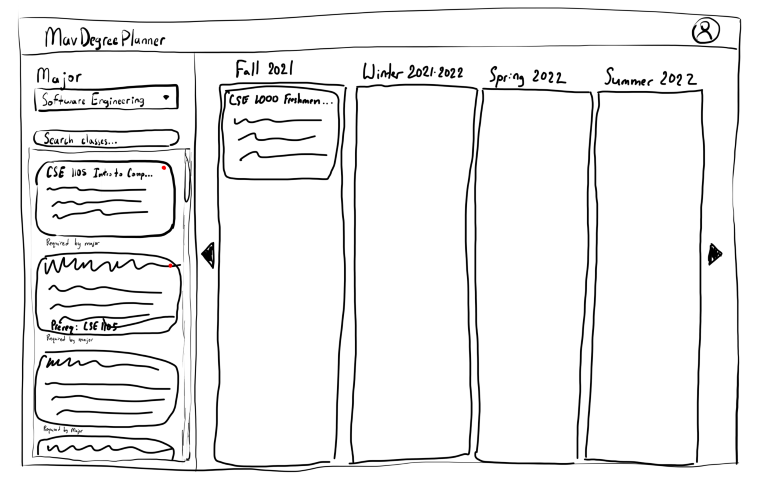
\includegraphics[width=0.60\textwidth]{images/MavDegreePlannerDiagram-Small}
\end{figure}
% End image insertion ------------------
\vspace{0.5 in}
{\centering \huge \color{accentcolor} \sc \textbf{\teamname \\ \productname} \par}
\vspace{0.5 in}
{\centering \large \sc \textbf{\authors} \par}
\newpage


%\vspace{1 in}
%\centerline{January 13th, 2012}
%\newpage

%%% Revision History
%%%%%%%%%%%%%%%%%%%%%%%%%%%%%%%%%%%%%%%%%%%%%%%%%%%%%%%%%%%%%%%%%
% Each '\vhEntry' begins a new version entry, and each {} is a 
% column. Update this to reflect your version history.
\begin{versionhistory}
  	\vhEntry{0.1}{10.12.2021}{Ijaz,Daniel,Safi,Le}{document creation}
\end{versionhistory}
\newpage

%%% Table of contents
\tableofcontents
\newpage

%%% List of figures and tables (optional)
\listoffigures
%\listoftables
\newpage
\setcounter{table}{0}

%%% Executive summary sections
% The \section command creates a section, assigns it a number and gives it the title in the braces.
% The \input command inserts the contents of the text file indicated in the braces.
\section{Problem Statement}
Many students at UTA come in and have a hard time following the degree plan that is given to them by their adivisors. If the students had a way to track their progress and know what stage they are at in their degree plan, then it can help make it easier for them to graduate and complete their degree plan. In addition, advisors have a tough job and they are busy a lot. This degree planner can help take the load off advisors and give the students an alternate way to plan their degree plan without having to wait for advisors to respond or to meet with them on their scheduled data. Finally, the degree plan will allow to students to even adjust their plan. Wether they want to take extra classes or if they want to graduate early the degree planner will help them calculate that and give them an illustration of what they would have to do to meet their timeline. 

\section{Methodology}
We are going to build an app that will help students plan their classes. It will give them the option to drag and drop classes, and this way they can make their degree plan. It will be interactive as in if the students select a class that requires another class then they wont be able to add that ahead of the class that is the pre req. It will also be able to handle co req so that they can take that class and a higher level class at the same time. This will help mitigate students that are confused about which classes they need next and it will help plan their college degree better. 
\section{Value Proposition}
This project will make it much easier for Freshman students to plan out their degrees.

The University will benefit from this because Advisors will be able to spend less time
    planning degree plans for students because they will be able to do it themselves easily.
    Advisors can also use this project to quickly check if a student's request classes are
    missing any pre-reqs or co-reqs.
\section{Development Milestones}

%%%%%%%%%%%%%%%%%%%%%%%%%%%%%%%%%%%%%%%%%%%%%%%%%%%%%%%%%%%%%%%%%%%%%%%%%
% This creates a bullet list. To add a bullet, use the \item command.
% Make sure it is between the \begin{itemize} and \end{itemize} commands.
\begin{itemize}
  \item Project Charter first draft - October 2021
  \item System Requirements Specification - October 2021
  \item Architectural Design Specification - November 2021
  \item Demonstration of Accounts and Project Setup - January 2022
  \item Detailed Design Specification - February 2022
  \item Demonstration of Database of Classes and List of Classes - February 2022
  \item Demonstration of Columns Per Semester that can hold classes - March 2022
  \item CoE Innovation Day poster presentation - March 2022
  \item Demonstration of Drag and drop classes into semester columns - April 2022
  \item Demonstration of Validate class prereqs and coreqs for classes in columns - April 2022
  \item Final Project Demonstration - May 2022
\end{itemize}

\newpage

%%% Remaining project charter sections
\section{Background}
The reason behind taking up this project is that the current UTA degree planner is not user friendly nor does it give users an interactive environment to easily choose their classes. Users need to be able to easily choose classes to plan out their classes to finish their degree in a timely manner. The best way to do that is to eliminate any confusion while users plan it out. This is why we chose this project, since as students we also understand the need of a proper degree planner, which checks if prerequisites are met, let the user know if they're missing something, and overall a easy User Interface to plan out the classes. Moreover, as former freshman students, we understand the confusion that there maybe in knowing what classes can I take this semester and finding the flowchart hard to follow, therefore, the goal of this app is to aid to the needs of these new students and give them a solid idea of how to plan out their four year degree, and give them the confidence as they would know that they are on track.\\

The customer of this project is Professor Chris Conly. He wants us to work on this project because he feel's that an interactive degree planner with options such as drag and drop, will help users visualize their classes much easily than the traditional one. Furthermore, as our professor and the students are Computer Science and Engineering students, the focus of the degree planner will be to specifically meet the needs of those students alone, so that this project can be feasible.
\section{Related Work}
%%%%%%%%%%%%%%%%%%%%%%%%
% To cite something, use the \cite command with the name of the bibtex entry in the curly braces.
% It will determine which reference number it is and insert that number where the \cite command is.
% e.g. \cite{Rubin2012}

According to Dr. Yusuff in his peer-reviewed article "Does personalized goal setting and study planning improve academic performance and perception of learning experience in a developing setting?", the goal setting and study planning contributes substantially to the academic performance \cite{YUSUFF2018232}. With this in mind, the comprehensive academic plan from the beginning of college life is essential for students to understand their expectations, interests, and future opportunities. Following this, the purpose of this project is to help students perform their academy at the highest standard. Also, it aims to assist the Department of Advisors in eliminating paperwork and optimizing the advising process. The Interactive Degree Planner allows students to log in using their netIDs. The web page will display the the list of courses that allows user to drag and drop desired item to each semester. However, the course option is only available when its pre-/co-requisite requirements are fulfilled. As long as the course is added into the semester box, the total hours/credits taken that semester will be accordingly updated. The website is expected to assist students to achieve better acknowledgement about their career paths since it provides visualization and interaction, which is scientifically proved as "an excellent way to learn and master complex systems" \cite{bobek_creating_2016}.
With respect to the currently existing application that share the similar ideas with this project, Prepler is the popular web-based degree planner among many colleges \cite{prepler_prepler_nodate}. It is free for basic feature and presents a simple interface. Ellucian Degree Works is the more advanced application compared to Prepler, which offers services in wide range of field from education to business \cite{noauthor_unifying_nodate}. Since Ellucian's application is overloaded with several functionalities using latest technology, this may impact negatively in user experience \cite{noauthor_improve_nodate}. Overall, there are a tons of analogous applications that are commercially available nowadays. Nevertheless, they do not offer the high-quality of visualization (e.g., degree flowchart, curriculum sheet, etc.) as this project intended to provide. That is to say, instead of dragging and dropping courses on the interactive interface, students must manually search or enter the course information to the planner. This requires them to familiarize themselves with the degree requirements, which is challenging, especially for freshman students. In fact, these applications focus on degree auditing rather than solely planning; henceforth, they may not support the user-friendly interfaces. Another key point is that they are not applicable specifically to UTA degree planner, which can be implemented practically at campus-wide level.
\section{System Overview}
The website will consist of a side panel with a list of classes and the main
    screen with columns for each semester. It will also have a section for user accounts.

The user can sign up for an account to access their plan anywhere. The system
    will support signin, signout, and forgot password. The system will collect email and
    password for signup and signin.

The side panel lists all classes available to a student. At the top of the side panel,
    the user can choose their major to check their classes against for pre/coreqs.
    Classes required by a student's major will be shown at the top, other classes
    will be at the bottom. It will show required classes that have satisfied
    the prereq and coreq requirements at the top of the list required classes section.
    The list of classes is also searchable. The major and chosen classes are saved
    to the user's account so they can access it later.

The main screen consists of a horizontably scrollable list of semesters. Each
    semester has a list of classes that the user has chosen. The first semester
    shown on the screen is the current one.

Each class can be dragged from the side panel to a semester's list of classes.
    The class will have an error above it if the user has not taken a prereq/coreq class
    in a previous semester, or if the user has not chosen a coreq in the same
    semester.
    
\begin{figure}[h!]
    \centering
    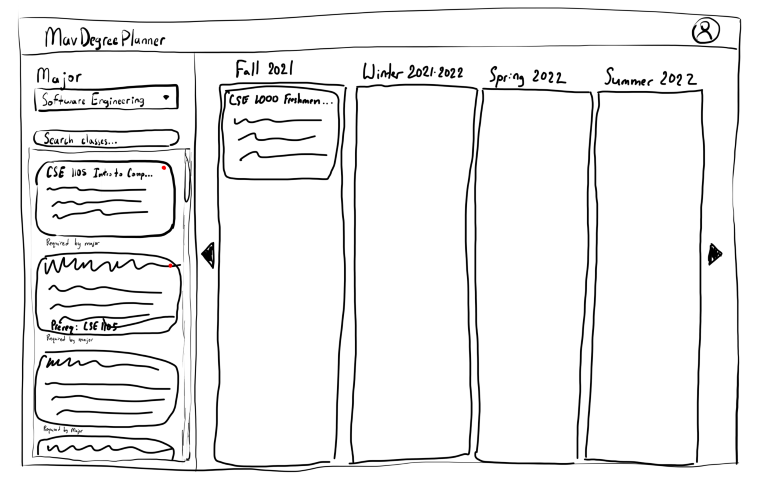
\includegraphics[width=0.5\textwidth]{images/MavDegreePlannerDiagram-Small} % Image
    \caption{Diagram of Major System Components} % Caption
\end{figure}
\section{Roles \& Responsibilities}
The stakeholders are Professor Conly and Professor Mcmurrough. The point of contact will be from our team to Professor Conly. If there is anything that needs to be communicated to Professor Mcmurrough it will be done by our team members to professor mcmurrough or it will go through Professor Conly. 

The team members and their respective roles are:

    Safi Ullah- front end
    
    
    Ijaz Umar-front end
    
    
    Daniel Newville-backend
    
    
    Le Uyen Nguyen-backend
    
    Right now the roles arent finalized, however we are all working together to see if anybody wants a different role that they will be better suited in. 
    The responsibilities are simple. Everyone must work on parts that contribute to the project. We are going to meet up and divide up the work together and once that is done we will set a timeline for when we want the work done. Usually the deadline will be a couple days ahead of the last day of the sprint, that way we can iron things up. We will try our best to communicate with one another and make sure that we dont fail to mention any details that may be vital to the success of the project. 
\section{Cost Proposal}
The project mainly focuses on building a web-based application, which relies on software, database, and networking tools. The budget of building the website can be broken down into two fundamental components: a home, which is the web domain, and an infrastructure, which is the web hosting. We plan to buy the domain name when the project is done at the end of the semester. To build the more practical website, the web hosting will consume most of the budget.

\subsection{Preliminary Budget}
Include a high level budget table for components, fabrication, software licensees, development hardware, etc.

\begin{center}
\begin{tabular}{||c | c | c ||} 
 \hline
   & Item Description & Estimated Cost \\ [0.5ex] 
 \hline\hline
 1 & Web Domain Name & \$20 \\ 
 \hline
 2 & Web Hosting & \$50 - \$300  \\ 
  \hline
 3 & Poster & \$40  \\ [1ex] 
 \hline
\end{tabular}
\end{center}

\subsection{Current \& Pending Support}
All of the funding source for the project comes from \$800 budget provided by the UTA CSE department. There is no current external funding. Any change made will be updated in this document accordingly.
\section{Facilities \& Equipment}
Since the project is solely a web-based application, we do not require any hardware, but computers connected to the high-speed Internet would be mandatory. Any testing in this project will be implemented on these devices. In light of lab space, due to the Covid-19 situation, in the beginning phase of this project, we do not plan to meet physically in-person. All meetings in this phase is transitioned to virtual on Discord platform. In case the pandemic is officially under control and there is no possibility of infection endangering team members' health and wellness, the UTA's laboratory located in Room 208, 202, and 203 on the second floor of the Engineering Research Building (ERB) will be used for holding any in-person meeting. For this project particularly, we will need the domain name for the website. There are multiple domain registrars that offer the domain name at low cost per month or per year. Once the website is fully or almost done, we will choose the most appropriate domain name from the reliable provider. Besides, the database plays a key role in this project. It would be ideal that UTA can give us access to the CSE department database in order to build the most practical and up-to-date application. Otherwise, we plan to simulate our own database to solely serve the purpose of developing this project. It may take a considerable effort to build the close-to-real-life database, but it will be free. Additionally, we also require the web hosting. Many reputable companies, such as AWS, Microsoft, and Google, provide several packages for hosting the website. The price may vary depending on the website's expectations and goals. We plan to have the special meeting thoroughly discussing this issue when it is appropriate. By the same token, we need the web design software tools for this project. Currently, we plan to use the open-source framework, which is also free. At the end of this project, it is necessary for the team to prepare a poster introducing the project. The plotter printer is available at multiple locations on campus that can fulfil this task. 
\section{Assumptions}
The following list contains critical assumptions related to the implementation and testing of the project.

%%%%%%%%%%%%%%%%%%%%%%%%%%%%%%%%%%%%%%%%%%%%%%%%%%%%%%%%%%%%%%%%%%%%%%%%%
% This creates a bullet list. To add a bullet, use the \item command.
% Make sure it is between the \begin{itemize} and \end{itemize} commands.
\begin{itemize}
  \item We will assume all classes are available to take if it is in the flowchart for that specific major.
  \item We will primarily be coding in React JS and using Firebase as the database.
  \item Will use the latest available flowchart as guide to the degree planner no matter when the student started pursuing their degree
  \item We will assume the professor will be available to validate system design and features.
  \item There won't be a need for buying any components as this is purely a software based project.
\end{itemize}
\section{Constraints}
The following list contains key constraints related to the implementation and testing of the project.

%%%%%%%%%%%%%%%%%%%%%%%%%%%%%%%%%%%%%%%%%%%%%%%%%%%%%%%%%%%%%%%%%%%%%%%%%
% This creates a bullet list. To add a bullet, use the \item command.
% Make sure it is between the \begin{itemize} and \end{itemize} commands.
\begin{itemize}
  \item The degree plan will be only for CSE students so that the project can be feasible.
  \item App will not update what classes user has taken previously as that would be done manually by the user, since we won't have access to such data.
  \item Need to make this app only web/desktop specific and not multi-platform due to time constraint
  \item We will be manually entering the data for the degree planner without access to the UTA database.
  \item Will need to start designing the database and logic for implementing the features of the application by end of Senior Design 1 to stay on schedule.
\end{itemize}

\section{Risks}

%%%%%%%%%%%%%%%%%%%%%%%%%%%%%%%%%%%%%%%%%%%%%%%%%%%%%%%%%%%%%%%
% This is the table. To add a row, separate each column with an
% ampersand (&) and end the line with the \hline command.
\begin{table}[h]
\resizebox{\textwidth}{!}{
\begin{tabular}{|l|l|l|l|}
\hline
 \textbf{Risk description} & \textbf{Probability} & \textbf{Loss (days)} & \textbf{Exposure (days)} \\ \hline
 Programmers not learning the required framework on time  & 0.50 & 30 & 15 \\ \hline
 Team member falling sick due to COVID-19  & 0.20 & 10 & 2 \\ \hline
 Not being able to implement some features on time  & 0.25 & 20 & 5 \\ \hline
 Not making the UI user friendly  & 0.15 & 20 & 3 \\ \hline
 Not being able to get the required data for implementation  & 0.10 & 15 & 1.5 \\ \hline
\end{tabular}}
\caption{Overview of highest exposure project risks} 
\end{table}
\section{Documentation \& Reporting}
%%% In this section, you will describe all of the various artifacts that you will generate and maintain during the project life cycle. Describe the purpose of each item below, how the content will be generated, where it will be stored, how often it will be updated, etc. Replace the default text for each section with your own description. Reword this paragraph as appropriate.

\subsection{Major Documentation Deliverables}

\subsubsection{Project Charter}
The project charter will be updated at the end of each sprint if necessary. The circumstance in which this document will be updated is based off the sprint review, and we as a team will check if there is a change in any aspect of our project, and will update accordingly. The initial version will be delivered October 11th, 2021. The final version will be delivered at the beginning of May 2022.

\subsubsection{System Requirements Specification}
This document will be updated after the discussion with team members and sponsor about the product requirements, and/or when there is any change in current requirements or addtion of new features. The initial version will be delivered at the end of October 2021, and the final version will be delivered in May 2022.

\subsubsection{Architectural Design Specification}
The document's initial version will be delivered November 15, 2021. The final version will be delivered in May 2022.

\subsubsection{Detailed Design Specification}
This document will be maintained and updated as we continue to develop the web application. If we make any change in the software functionality then we will update this accordingly. The document's initial version will be delivered at the end of February 2022. The final version will be delivered in May 2022. 

\subsection{Recurring Sprint Items}
The following items will be documented and maintained during each individual sprint.

\subsubsection{Product Backlog}
All requirements and update that are collected during the discussion between team members and Professor Chris Conly/sponsor will be added to the product backlog from the SRS. The items will be prioritized based on its urgency of getting feedback and the relation to other items. However, in case the sponsor prioritizes any feature, the hierarchy may be change accordingly. Any decision on the project will be decided based on group vote and the sponsor's advice. We will use GitHub to maintain and share the product backlog with team members and stakeholders.

\subsubsection{Sprint Planning}
Each sprint will be planned following the end of the previous sprint during a meeting with all team members. There will be eight sprints.

\subsubsection{Sprint Goal}
The sprint goal will be decided by the team as a whole. The team can meet with the customer for feedback, or the sprint plan will be emailed to them for feedback.

\subsubsection{Sprint Backlog}
The team leader and their assistent will choose which product backlog items make their way into the sprint backlog. GitHub Projects will be used to maintain the backlog items.

\subsubsection{Task Breakdown}
Each team member will voluntarily claim their tasks, and they will also document the time spent on each task in their Engineering Notebook.

% \subsubsection{Sprint Burn Down Charts}
% Who will be responsible for generating the burn down charts for each sprint? How will they be able to access the total amount of effort expended by each individual team member? What format will the burn down chart use (include an example burn down chart below).

% %%%%%%%%%%%%%%%%%%%%%%%%%%%%%%%%%%%%%%%%%%%%%%%%%%%%%%%%%%
% %  BE SURE TO UPDATE THE IMAGE CAPTION
% \begin{figure}[h!]
%     \centering
%     
\includegraphics[width=0.5\textwidth]{images/test_image} % Image
%     \caption{Example sprint burn down chart} % Caption
% \end{figure}

\subsubsection{Sprint Retrospective}
The team will meet and document everything that was done between the team members. The disussion will happen before the next sprint starts. Every feature will be sorted by which group members worked on it, and if multiple members worked on an item or was worked on during a group meeting. This will be due before the start of each sprint.

\subsubsection{Individual Status Reports}
We will create the individual Status Report based off the sample report provided by the professor. It will be reported at the end of each sprint. The report will contain the spring goal, sprint backlog, individual time expenditures, individual retrospective, a peer review, and if needed a burndown chart. 

\subsubsection{Engineering Notebooks}
The Engineering Notebook will be updated by each member at the end of the day that they worked on the project. The minimum amount of pages will vary per sprint. Each interval is a week long. The team will keep each member accountable by reminding everyone to update their ENB at the end of every week. Any teammate that is available can sign off as a "witness" for each ENB page.

\subsection{Closeout Materials}
The following materials, in addition to major documentation deliverables, will be provided to the customer upon project closeout.

\subsubsection{System Prototype}
There will be a working web application where users will be able to make their own degree plan. The PAT and FAT will be decided later on as we start developing the project.

\subsubsection{Project Poster}
The project poster will be devlivered at the mid-March 2022. The final dimensions will be decided when the poster is being created. The poster as of now will include pictures of the web application, and will be designed in a manner where the viewers will be able to get a better understanding of the features provided by our application.

\subsubsection{Web Page}
Our project is the web-based application that is accessible to public, therfore, the homepage will basically be the project home page. The final product will be delivered at the end of semester in May 2022.

\subsubsection{Demo Video}
The demo video will be a sreen recording of the web application in use. The demo will create a sample user and show how to use the application and create a degree plan. 

\subsubsection{Source Code}
The source code will be maintained using Git and GitHub. Source code will be provided to the customer as a ZIP file. The project will also be open source with the license GPL-3.0. The lisense terms are listed in a file called "LICENSE" in the source code ZIP file.

\subsubsection{Source Code Documentation}
Documentation will be required for all classes, methods, functions, and variables. A documentation generator will be used, a specific tool will be decided on at a later time. The format of the final documentation will decided later.

\subsubsection{Hardware Schematics}
The project is fully web-based application, so we do not require any hardware schematics.

\subsubsection{CAD files}
The project is fully web-based application, so we do not require CAD files.

\subsubsection{Installation Scripts}
There will be a readme file with instructions and screenshots. Perhaps even some copy and
    paste lines for installation.

\subsubsection{User Manual}
A digital user manual and a demo video explaining all instructions will be available for the customer.

\newpage

%%% References
\bibliographystyle{plain}
\bibliographystyle{reference/IEEEtran_custom}
\bibliography{reference/refs}{}

\end{document}